%%%%%%%%%%%%%%%%%%%%%%%%%%%%%%%%%%%%%%%%%%%%%%%%%%%%%%%%%%%%%%%%%
%
% Project     : Bachelorarbeit
% Title       : Machbarkeitsanalyse für eine ressourcenorientierte Schnittstelle zur Verarbeitung grundlegender Probleme der Informatik
% File        : umsetzung.tex Rev. 01
% Date        : 01.03.2015
% Author      : Raffael Santschi
%
%%%%%%%%%%%%%%%%%%%%%%%%%%%%%%%%%%%%%%%%%%%%%%%%%%%%%%%%%%%%%%%%%

\chapter{Umsetzung des Prototyps \resultAssignment{[R5]}}\label{chap.umsetzung}
In diesem Kapitel wird kurz auf die Erkenntnisse aus dem \glslink{vertikaler_durchstich}{vertikalen Durchstich} eingegangen. Danach wird erklärt, wie die Umsetzung für die ausgewählten 
Problemtypen durchgeführt wurde. Zu guter Letzt wird noch die Entwicklungsumgebung für dieses Projekt beschrieben.

\section{Erster Durchstich}\label{entwicklungsumgebung}
Zum Start der Umsetzung wurde ein erster \gls{vertikaler_durchstich} anhand des Rucksack-Problems gemacht, um zu sehen, ob sich das Konzept bewährt. Während der 
Implementation wurde bereits überlegt, wie die Logik möglichst generisch gehalten werden kann.

\begin{figure}[h]
\centering
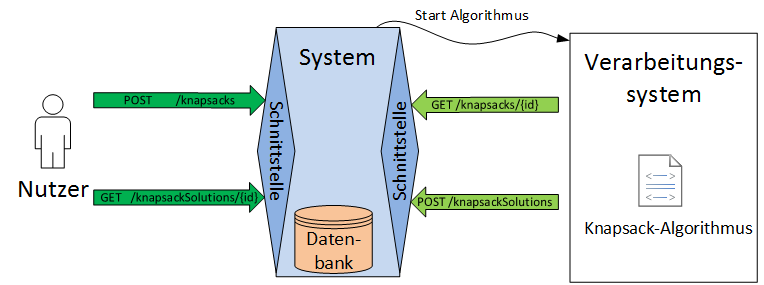
\includegraphics[scale=0.74]{images/visio/prototype_knapsack.png}
\caption[\Gls{vertikaler_durchstich} mit dem Rucksack-Problem]{Vertikaler Durchstich mit dem Rucksack-Problem \selfmade{}}
\label{fig:prototyp_knapsack}
\end{figure}

\subsection{Erkenntnisse nach dem ersten Durchstich}\label{learning_prototyp}
Die Kontaktschnittstelle zum Nutzer generisch zu halten, macht aus Gründen der Benutzerfreundlichkeit keinen Sinn. Für den Kunden ist es transparenter, wenn er eine Schnittstelle aufruft, 
welche zum Beispiel 'timetableComputations' heisst, statt einer generischen Schnittstelle namens 'computations'. Zudem ist es nicht möglich nur mithilfe der Daten herauszufinden, welches 
Problem gelöst werden möchte. Dazu würde es einen zusätzlichen Parameter benötigen. Weiter stellt es sich als schwierig heraus, mit Spring einen Endpunkt bereitzustellen, welcher 
verschiedene Ressourcentypen akzeptiert. Die Validierung der Eingabeparameter würde dadurch zusätzlich erschwert werden.

Das Konzept mit den beiden Translators bietet sehr viele Möglichkeiten und Flexibilität. Es entkoppelt die Nutzer-Schnittstelle komplett von der Schnittstelle für die Algorithmen. Um diese 
Flexibilität ausnutzen zu können, müssen jedoch oft verschiedene Entities für die Nutzer- und Algorithmus-Sicht erstellt werden.

In der Business Logik kann vieles allgemein gehalten werden. Die Repositories, Services und die Interfaces können generisch programmiert werden und bleiben für alle Probleme gleich. Beim 
Controller kann die Logik in einer abstrakten Klasse definiert werden. Somit müssen nur noch die Namen der Schnittstellen in der spezifischen Implementation definiert werden. Es hat sich 
gezeigt, dass sich das Konzept bewährt und die weiteren Probleme dementsprechend gelöst werden konnten.

\subsection{Anpassung des Konzepts nach dem ersten Durchstich}\label{doings_prototyp}
Das Konzept wurde nach dem ersten \glslink{vertikaler_durchstich}{Durchstich} dahingegen geändert, dass die Schnittstellen auf der Nutzer-Seite umbenannt wurden und die 
Algorithmus-Seite einen anderen Namespace erhielt. Weiter verschwand die separate Schnittstelle für das Abfragen des Resultats, die Funktionalität wurde stattdessen in die Status-Abfrage 
integriert.

\section{Implementierung der Schnittstelle}\label{impl_interface}
In diesem Abschnitt wird über die Implementation der Schnittstelle im Allgemeinen geschrieben. Wie bereits erwähnt ist der Ablauf bei jedem Problem gleich, dementsprechend verhält sich die 
Schnittstelle auch sehr ähnlich.

\subsection{Statusabfrage}
Damit der Nutzer möglichst wenig Schnittstellen ansprechen muss, erhält er bei einer Statusabfrage ebenfalls die vorhandenen Resultate. Der Nutzer erhält nur Resultate mit dem Status 'FINAL'. 
Resultate mit dem Status 'PARTIAL' werden zwar beim Status und der Zeit des zuletzt empfangenen Resultats berücksichtigt, aber nicht herausgegeben. Der Status besitzt neben den 
Resultaten eine ID und einen Namen, weiter werden Startzeit, Endzeit und die Zeit des zuletzt empfangenen Resultats angegeben. Falls eine Berechnung beendet ist, wird eine 
Begründung der Beendigung angezeigt. Dies kann zum Beispiel ein aufgetretener Fehler während des Starts oder der Berechnung sein oder eine Bestätigung der erfolgreichen Berechnung.

\begin{lstlisting}[language=JSON, caption=Aufbau einer Antwort auf eine Statusabfrage, label=lst:status_response]  
{
  "id'': "<Berechnung ID>",
  "name": "<Berechnungsname>",
  "computationStatus": "<Status der Berechnung>",
  "createDate": <Erstelldatum>,
  "finishDate": <Enddatum>,
  "finishedReason": "<Begruendung der Beendigung>",
  "lastResultReceived": <Datum des zuletzt empfangenen Resultats>,
  "solutions": <Resultate>
}
\end{lstlisting}

\subsection{WebHook Möglichkeit}
Die Berechnungen können je nach Komplexität sehr lange dauern. Der Nutzer müsste immer wieder den Status abfragen, um zu sehen, ob ein Resultat vorhanden ist. \glspl{webhook} 
bieten Abhilfe für dieses Problem. Das Verfahren ist nicht standardisiert, es ist aber sehr simpel und hilfreich. Beim Start einer Berechnung kann eine URL mitgegeben werden, zu welcher 
bei jeder Statusänderung ein POST-Request gesendet wird. Um diese Schnittstelle möglichst generisch zu halten, wurde eine Möglichkeit geschaffen, eine beliebige Payload für den 
POST-Request anzugeben. Die Nachricht der Statusänderung kann nach belieben mit dem Platzhalter '\_\_MESSAGE\_\_' irgendwo in die Payload eingebunden werden. Das Attribut 'message' 
wird in der Nachricht gesetzt, wenn der Platzhalter nirgends verwendet wird. Eine Konfiguration für die Chat-Applikation 'Slack' würde wie in \autoref{lst:webhook_configuration} 
aussehen. Die Nachrichten bei Statusänderungen sähen dann wie in \autoref{fig:slack_chat} aus.

\begin{lstlisting}[language=JSON, caption=Beispiel einer WebHook Konfiguration für Slack, label=lst:webhook_configuration]
  ...  
  "webHookConfiguration": {
    "url": "https://hooks.slack.com/services/T0000/B0000/XXX",
    "payload": {
        "text": "__MESSAGE__",
        "channel": "#simplatyser",
        "username": "simplatyser",
        "icon_emoji": ":squirrel:"
    }
  }
 ...
\end{lstlisting}

\begin{figure}[h]
\centering
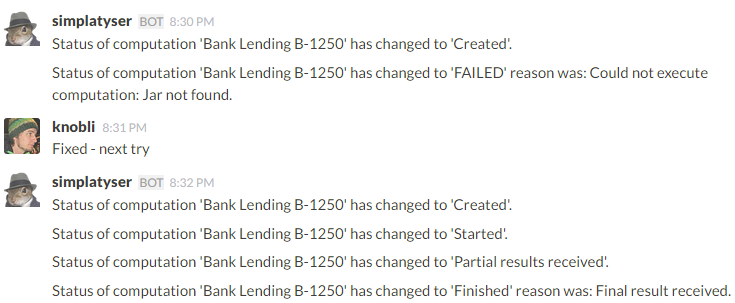
\includegraphics[scale=0.8]{images/slack_chat.png}
\caption[Nachrichten der Statusänderungen von Berechnungen]{Nachrichten der Statusänderungen von Berechnungen \selfmade{}}
\label{fig:slack_chat}
\end{figure}

\subsection{Technische Umsetzung und Herausforderungen}
Das Fundament der Software war mit Spring Boot \cite{spring_boot} sehr schnell gebaut, die Anbindung an MongoDB wurde mit Spring Data \cite{spring_data} realisiert. Leider war 
oftmals die Dokumentation nicht ausreichend oder nur für die XML-Konfiguration von Spring ausgelegt. Weiter gab es fehlende Teile in Spring Data, welche gefunden werden mussten. 
So gibt es zum Beispiel zu diesem Zeitpunkt standardmässig keine Möglichkeit, ein 'LocalTime'-Objekt oder ein 'LocalDateTime'-Objekt von Java 8 zu persistieren. Dies führte zu einem 
Stackoverflow anstatt einer spezifischeren Exception, was wiederum die Suche nach dem Fehler erheblich erschwerte. Um diese Probleme zu beheben, musste ein eigener Converter 
geschrieben und dieser bei der MongoDB-Konfiguration angegeben werden.

Bei der Business Logik wurde darauf geachtet, dass vieles mit \gls{generics} gelöst werden konnte. Vor allem bei den Services konnte viel Code für alle Probleme wiederverwendet werden. Auch 
bei den beiden Scheduling-Problemen konnte viel Code-Duplizierung vermieden werden. Zusätzlich wurden häufig verwendete Funktionen, wie das Abbilden auf die Input-Objekte, in 
Helfer-Klassen ausgelagert, damit sie nur ein Mal implementiert werden mussten.

\section{Implementierung der Probleme}\label{impl_problems}
In diesem Unterkapitel wird für jedes Problem kurz erklärt, was beim Prototyp implementiert wurde, um die Möglichkeiten des Konzepts aufzuzeigen. Eine ausführliche 
Schnittstellen-Dokumentation ist in \autoref{api_doc} zu finden. Zusätzlich wurde noch eine elektronische Dokumentation der Schnittstelle mit Hilfe von Swagger UI \cite{swagger} erstellt. 
Diese stellt die angebotenen Schnittstellen, die Eingabeparameter und die Resultat sehr übersichtlich dar.

\begin{figure}[h]
\centering
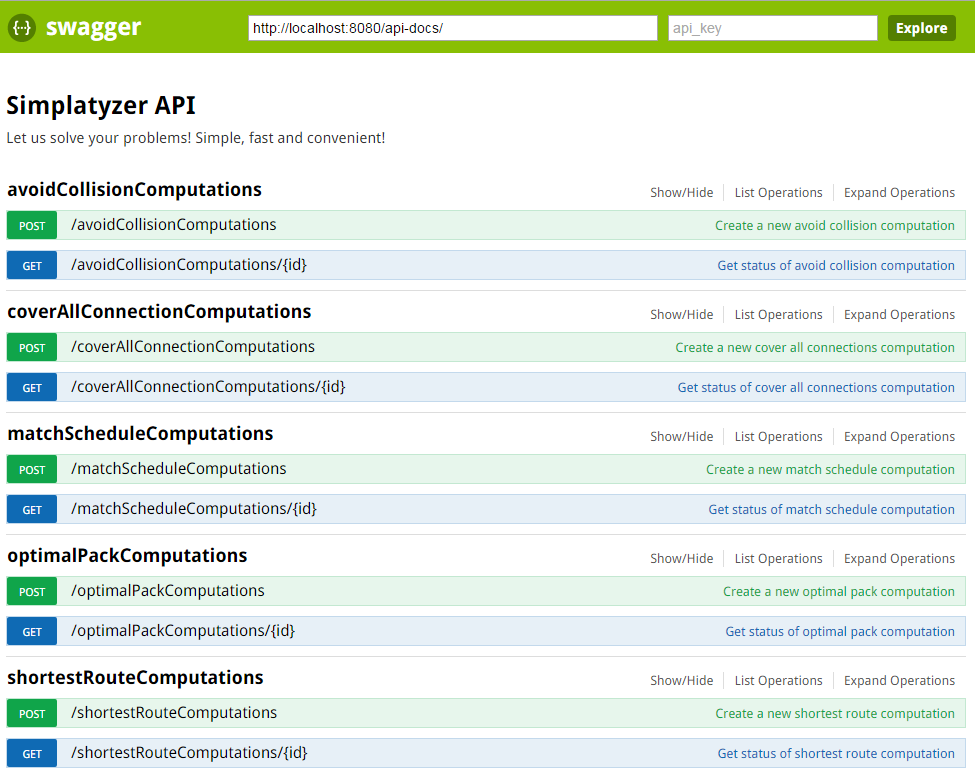
\includegraphics[scale=0.5]{images/swagger_api.png}
\caption[Nutzer-Schnittstellenbeschreibung von Swagger]{Nutzer-Schnittstellenbeschreibung von Swagger \selfmade{}}
\label{fig:swagger}
\end{figure}

\FloatBarrier

Beim Evaluieren des Stundenplan-Problems wurde bemerkt, dass es sehr viele verschiedene Planungsprobleme gibt. Deshalb wurde ein zusätzliches Planungsproblem gewählt, 
um zu schauen, wie sich die Schnittstelle bei sehr ähnlichen Problemen verhält.

%%%%%%%%%%%%%%%%%%%%%%%%%%%%%%%
%
%
%		Rucksack
%
%
%%%%%%%%%%%%%%%%%%%%%%%%%%%%%%%

\subsection{Rucksack}
Das Rucksack-Problem ist aus Sicht der Schnittstelle ein relativ einfaches Problem. Um die Benutzerfreundlichkeit zu verbessern, kann der Nutzer bei den Elementen eine Anzahl definieren und 
muss sie nicht doppelt angeben. Der Algorithmus hingegen bekommt eine Liste mit den einzelnen Elementen. Zudem wird der Name der Element nicht weitergegeben, da er vom 
Algorithmus nicht benötigt wird. Der Algorithmus liefert als Resultat eine Liste von booleschen Werten zurück, diese müssen zuerst wieder auf die ursprünglichen Elemente abgebildet werden. Bei 
der Validierung wird überprüft, ob die Gewichtsschranke nicht überschritten wurde und ob ein Element nicht zu oft verwendet wurde. Letzteres ist zwar beim getesteten Algorithmus nicht 
möglich, könnte jedoch bei einer anderen Implementation der Fall sein. Der Benutzer erhält als Resultat eine Liste mit allen Objekten, welche verwendet wurden. Wenn ein Objekt mehrmals 
verwendet wurde, wird die entsprechende Anzahl angegeben.

\begin{figure}[h]
\centering
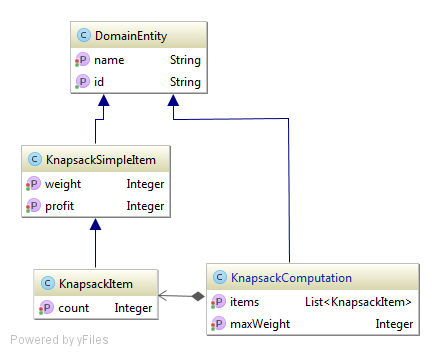
\includegraphics[scale=0.5]{images/probleme/knapsack.png}
\caption[Eingabeparameter für eine Rucksack-Berechnung]{Eingabeparameter für eine Rucksack-Berechnung \selfmade{}}
\label{fig:knapsack_input}
\end{figure}

\FloatBarrier

%%%%%%%%%%%%%%%%%%%%%%%%%%%%%%%
%
%
%		Knotenfärbung
%
%
%%%%%%%%%%%%%%%%%%%%%%%%%%%%%%%

\subsection{Knotenfärbung}
Bei der Knotenfärbung geht es darum, Kollisionen zu vermeiden. Dies wurde für den Nutzer möglichst transparent umgesetzt. Der Nutzer kann mögliche Werte (z.B. Farben oder 
Frequenzen) angeben, welche die Elemente zugeteilt bekommen sollen. Der Algorithmus erhält eine Liste mit allen Elementen und ihren Nachbarn. Die Namen der Elemente und die möglichen 
Werte werden nicht weitergegeben. Es wird davon ausgegangen, dass der Algorithmus eine Liste von Elementen mit den zugewiesenen Werten zurückgibt. Beim Übersetzen werden 
die Werte vom Algorithmus mit den möglichen Werten aus der Benutzereingabe ausgetauscht. Falls der Nutzer keine Werte angegeben hat, werden die Werte vom Algorithmus weitergegeben. 
Bei der Validierung wird überprüft, dass kein Element den gleichen Wert wie einer seiner Nachbarn hat. Als Resultat erhält der Benutzer eine Liste mit allen Elementen und ihren zugewiesenen 
Werten.

\begin{figure}[h]
\centering
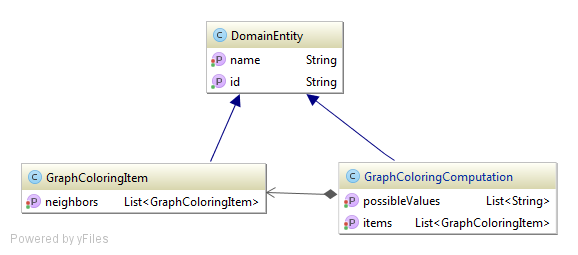
\includegraphics[scale=0.5]{images/probleme/graphcoloring.png}
\caption[Eingabeparameter für eine Knotenfärbung-Berechnung]{Eingabeparameter für eine Knotenfärbung-Berechnung \selfmade{}}
\label{fig:graphcoloring_input}
\end{figure}

%%%%%%%%%%%%%%%%%%%%%%%%%%%%%%%
%
%
%		Problem des Handlungsreisenden
%
%
%%%%%%%%%%%%%%%%%%%%%%%%%%%%%%%

\subsection{Problem des Handlungsreisenden}
Der Service bietet nicht nur die kürzeste Route für eine Liste von Wegpunkten an, es ist auch möglich, für jeden Wegpunkt eine gewünschte Ankunftszeit und Aufenthaltszeit anzugeben. Der 
Algorithmus erhält vom System eine Liste mit allen Wegpunkten, bei diesem Schritt wird nichts übersetzt. Es wäre jedoch theoretisch möglich, dass die Schnittstelle die Daten bereits für den 
Algorithmus aufbereitet, zum Beispiel indem sie die Kosten zwischen den Wegpunkten berechnet. Es wird davon ausgegangen, dass der Algorithmus eine Liste der Wegpunkte in der 
berechneten Reihenfolge zurückgibt. Beim Übersetzen werden die geplanten Ankunftszeiten berechnet, welche dann während der Validierung mittels der maximal angegebenen Abweichung 
überprüft werden. Der Benutzer erhält als Resultat eine Liste von Wegpunkten mit gewünschter und geplanter Ankunftszeit in der berechneten Reihenfolge.

\begin{figure}[h]
\centering
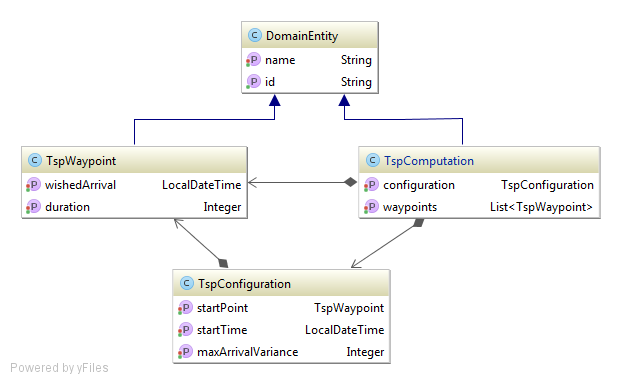
\includegraphics[scale=0.5]{images/probleme/tsp.png}
\caption[Eingabeparameter für eine Routen-Berechnung]{Eingabeparameter für eine Routen-Berechnung \selfmade{}}
\label{fig:tsp_input}
\end{figure}

%%%%%%%%%%%%%%%%%%%%%%%%%%%%%%%
%
%
%		Briefträgerproblem
%
%
%%%%%%%%%%%%%%%%%%%%%%%%%%%%%%%

\subsection{Briefträgerproblem}
Das Briefträgerproblem berechnet eine Route, welche alle bekannten Wege eines Graphen abfährt. Der Nutzer kann eine Liste von Wegpunkten mit den Verknüpfungen zu anderen 
Wegpunkten und ihrer Länge angeben. Der Algorithmus erhält vom System eine Liste mit allen Wegpunkten, die Namen der Wegpunkte werden nicht weitergegeben. Es wird davon ausgegangen, 
dass der Algorithmus eine Liste der Wegpunkte in der berechneten Reihenfolge zurückgibt. Beim Übersetzen werden die Wegpunkte wieder auf die Eingabewerte abgebildet und die komplette 
Länge der Route berechnet. Die Validierung überprüft, ob der Weg möglich ist und ob jede Verbindung mindestens ein Mal benutzt wurde. Der Benutzer erhält als Resultat eine Liste mit der berechneten 
Reihenfolge der Wegpunkte und die totale Länge der Strecke.

\begin{figure}[h]
\centering
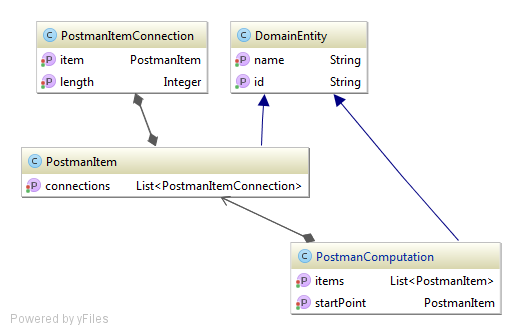
\includegraphics[scale=0.5]{images/probleme/postman.png}
\caption[Eingabeparameter für eine Briefträger-Routen-Berechnung]{Eingabeparameter für eine Briefträger-Routen-Berechnung \selfmade{}}
\label{fig:postman_input}
\end{figure}

\FloatBarrier
%%%%%%%%%%%%%%%%%%%%%%%%%%%%%%%
%
%
%		Stundenplan Erstellung
%
%
%%%%%%%%%%%%%%%%%%%%%%%%%%%%%%%

\subsection{Stundenplan Erstellung}
Das Erstellen eines Stundenplans ist ein Planungsproblem, welches sehr viele Möglichkeiten und Einschränkungen besitzt und somit sehr komplex ist. In dieser Implementation sind bei weitem 
nicht alle Spezialitäten abgedeckt. Es wurde darauf geachtet, dass bereits einige Einschränkungen, wie zum Beispiel freie Tage von Lehrern und blockierte Schulzimmer, miteinbezogen werden. 
Der Nutzer gibt eine Liste von Klassen, Lehrern, Schulzimmern und Schulfächern an. Die Klassen haben eine bestimmte Grösse und definieren auch, welche Fächer sie besuchen müssen. Die 
Lehrer haben eine Liste mit Schulfächern, welche sie unterrichten können, eine List mit zugehörigen Klassen und eine Definition ihrer freien Tage. Die Klassenzimmer besitzen eine Liste mit 
möglichen Schulfächern und eine Sperrliste, in welcher definiert ist, wann der Raum nicht verfügbar ist. Die Schulfächer können definieren, ob sie eine Raum brauchen, welcher explizit dafür 
bestimmt ist, zum Beispiel Sport in der Turnhalle. Neben den zu verplanenden Elementen gibt es Randbedingungen wie die Pausenzeiten, die Lektionsdauer und die Definition, 
wann unterrichtet werden soll. Der Algorithmus erhält eine Liste mit allen Klassen, Lehrern, Schulzimmern und Schulfächern. Die Rahmenbedingungen werden in Zeitfenster umgewandelt, 
welche vom Algorithmus verplant werden können. Zusätzlich werden die Elemente generischer benannt, damit der Algorithmus nicht verschiedene Konfigurationen für verschiedene 
Planungsprobleme besitzen muss. In \autoref{lst:cat_input_timetableScheduling} ist ein Beispiel für eine Eingabe der Rahmenbedingungen gezeigt, welche durch den Translator in die Zahl 36 
umgewandelt wird. Die Standard-Werte, welche mit dem Flag `defaultTimes' gesetzt werden, sind von 8:20 Uhr bis 17:10. Die Zahl wird aus der Lektionsdauer, den Pausen und den einzelnen 
Zeitfenstern pro Tag berechnet, die \autoref{table:timeslice_calc} stellt dies dar.

\begin{lstlisting}[language=JSON, caption=Ausschnitt einer Eingabe für das Stundenplanproblem für die Rahmenbedingungen, label=lst:cat_input_timetableScheduling]  
{
  ...
  "configuration": {
    "breakTimeSliceSize": [5, 20, 5, 90, 5, 20, 5],
    "dayTimeSlots": [
      {
        "monday": {"defaultTimes": true},
        "tuesday": {"defaultTimes": true},
        "wednesday": {"from": [8, 20, 0], "to": [12,0,0]},
        "thursday": {"defaultTimes": true},
        "friday": {"defaultTimes": true}
      }
    ],
    "lessonDuration": 45
  }
}
\end{lstlisting}

\begin{table}[ht]
\centering
  \begin{tabular}{ l | c | c | c | c | c }
	\hline
	\rowcolor{gray}
	\textbf{Uhrzeit} 	& \textbf{Mo}	& \textbf{Di} 	& \textbf{Mi}	&  \textbf{Do}	&  \textbf{Fr}\\ \hline
	0820-0905		& 1			& 9			& 17			& 21			& 29		\\ \hline
	0910-0955		& 2			& 10			& 18			& 22			& 30		\\ \hline
	1015-1100		& 3			& 11			& 19			& 23			& 31		\\ \hline
	1105-1150		& 4			& 12			& 20			& 24			& 32		\\ \hline \hline
	1320-1405		& 5			& 13			& -			& 25			& 33		\\ \hline
	1410-1455		& 6			& 14			& -			& 26			& 34		\\ \hline
	1515-1600		& 7			& 15			& -			& 27			& 35		\\ \hline
	1605-1650		& 8			& 16			& -			& 28			& 36		\\ \hline
  \end{tabular}
   \caption{Visuelle Darstellung der Zeitfenster-Berechnung}\label{table:timeslice_calc}
\end{table}

\begin{figure}[h]
\centering
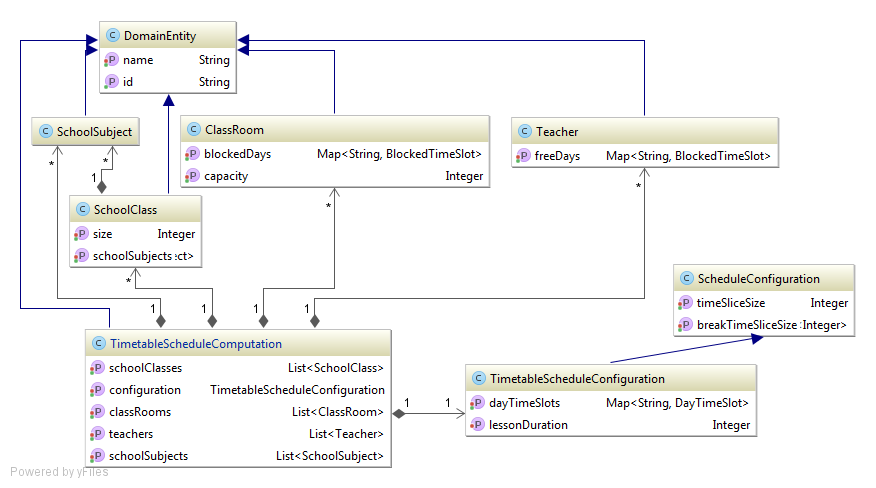
\includegraphics[scale=0.5]{images/probleme/timetableSchedule.png}
\caption[Eingabeparameter für eine Stundenplan-Berechnung]{Eingabeparameter für eine Stundenplan-Berechnung \selfmade{}}
\label{fig:timetableSchedule_input}
\end{figure}

\FloatBarrier

Es wird davon ausgegangen, dass der Algorithmus eine Liste von Planungskombinationen zurückgibt. Eine Kombination besteht aus einer Zeitfensternummer, einem Lehrer, einer Klasse, 
einem Schulfach und einem Klassenzimmer. Beim Übersetzen werden die IDs auf die ursprünglichen Elemente abgebildet, die Zeitfensternummern wieder werden in Uhrzeiten umgewandelt. 
Zusätzlich wird eine Statistik für die Lehrer geführt. Bei der Validierung wird überprüft, ob ein Element zu einer Zeit mehrfach verplant ist, ob der Lehrer die nötigen Fähigkeiten hat und ob ein 
Klassenzimmer für das Fach ausgelegt ist. Das umgewandelte Resultat enthält eine Liste mit den berechneten Kombination, sortiert nach Wochentag und Uhrzeit. Die Lehrerstatistik zeigt, wie 
oft ein Lehrer ein bestimmtes Fach und wie viele Stunden er insgesamt unterrichtet.

%%%%%%%%%%%%%%%%%%%%%%%%%%%%%%%
%
%
%		Spielplan Erstellung
%
%
%%%%%%%%%%%%%%%%%%%%%%%%%%%%%%%

\subsection{Spielplan Erstellung}
Eine weitere Ausprägung des Planungsproblems ist das Erstellen eines Spielplans. Der Nutzer gibt eine Liste von Teams, Schiedsrichtern, Spielfeldern und Kategorien an. Die Teams gehören in 
eine bestimmte Kategorie. Die Schiedsrichter haben eine Liste mit Kategorien, welche sie leiten können, und eine Liste von Teams, zu welchen sie gehören. Die Spielfelder besitzen eine Liste mit 
möglichen Kategorien. Neben den zu verplanenden Elementen gibt es Randbedingungen wie die Spieldauer, die Startzeit und die Pausenzeiten. Der Algorithmus erhält eine 
Liste mit allen Teams, Schiedsrichtern, Spielfeldern und Kategorien. Zusätzlich werden die Elemente generischer benannt, damit der Algorithmus nicht verschiedene Konfigurationen für 
verschiedene Planungsprobleme besitzen muss.

\begin{figure}[h]
\centering
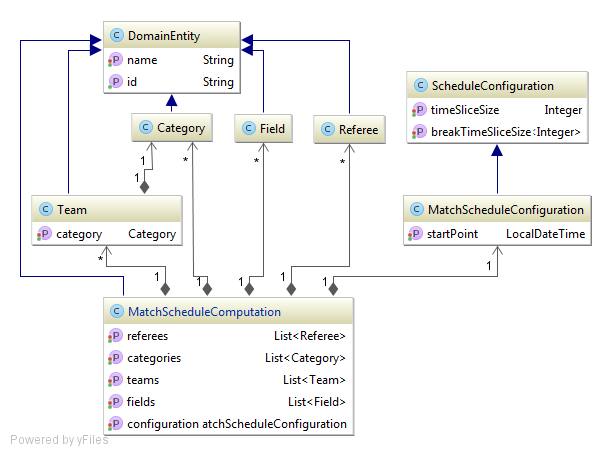
\includegraphics[scale=0.5]{images/probleme/matchSchedule.png}
\caption[Eingabeparameter für eine Spielplan-Berechnung]{Eingabeparameter für eine Spielplan-Berechnung \selfmade{}}
\label{fig:matchschedule_input}
\end{figure}

Es wird davon ausgegangen, dass der Algorithmus eine Liste von Planungskombinationen zurückgibt. Eine Kombination besteht aus einer Zeitfensternummer, einem Schiedsrichter, 
einer Kombination von zwei Teams und einem Spielfeld. Beim Übersetzen werden die IDs auf die ursprünglichen Elemente abgebildet und die Zeitfensternummern werden wieder in Uhrzeiten 
umgewandelt. Zusätzlich wird eine Statistik über die Einsätze der Schiedsrichter und der Teams geführt. Bei der Validierung wird beachtet, ob ein Element zu einer 
bestimmten Zeit mehrfach verplant ist, ob die Schiedsrichter die nötigen Fähigkeiten haben und ob ein Spielfeld für die Kategorie ausgelegt ist. Der Benutzer erhält als Resultat eine Liste 
mit den berechneten Kombination, sortiert nach Uhrzeit. Die Schiedsrichterstatistik zeigt, wie oft ein Schiedsrichter eine bestimmte Kategorie leitet und für wie viele Spiele er insgesamt 
verantwortlich ist. Die Teamstatistik zeigt, wie viele Spiele eine Kategorie insgesamt hat und wie viele Spiele ein Team bestreitet. In \autoref{lst:cat_result_matchScheduling} wird ein 
Ausschnitt der Schiedsrichterstatistik dargestellt.

\begin{lstlisting}[language=JSON, caption=Ausschnitt eines Resultats einer Spielplan Erstellung, label=lst:cat_result_matchScheduling]  
{
  ...
  name: "Sabine Pfister"
  statisticMap: {
    Knaben: 1
    Damen Kat A: 3
    Damen Kat B: 2
    _TOTAL: 6
  }
  ...
}
\end{lstlisting}

\subsection{Übersicht der Schnittstellen}
Für den Nutzer wurde ein problem-agnostischer Name für die Schnittstelle gewählt. Die Namen unterscheiden sich somit zum Teil zwischen Nutzer- und Algorithmus-Sicht. Damit die 
Verknüpfung der beiden Schnittstellen nicht verloren geht, und um eine Übersicht über alle angebotenen Schnittstellen zu haben, wurden sie in der \autoref{table:overview_api_interfaces} 
zusammengetragen. Die Endpunkte für die Algorithmen sind unter dem Namespace '/algorithm', damit diese beiden sauber voneinander getrennt sind.

\begin{table}[ht]
\centering
  \begin{tabular}{ l | l }
  	\hline
	\rowcolor{gray}
	\textbf{Nutzer}							& \textbf{Algorithmus}					\\ \hline
	/									& /algorithm/							\\ \hline
	\multicolumn{2}{|c|}{\textbf{Rucksack}}\\ \hline
	 POST /optimalPackComputations					& GET /knapsackComputations/\{ID\}			\\ \hline
	GET /optimalPackComputations/\{ID\}	& POST /knapsackComputations/\{ID\}/solutions	\\ \hline
	\multicolumn{2}{|c|}{\textbf{Knotenfärbung}}\\ \hline
	POST /avoidCollisionComputations				& GET /graphColoringComputations/\{ID\}		\\ \hline
	GET /avoidCollisionComputations/\{ID\}		& POST /graphColoringComputations/\{ID\}/solutions	\\ \hline
	\multicolumn{2}{|c|}{\textbf{Problem des Handlungsreisenden}}\\ \hline
	POST /shortestRouteComputations				& GET /tspComputations/\{ID\}				\\ \hline
	GET /shortestRouteComputations/\{ID\}		& POST /tspComputations/\{ID\}/solutions		\\ \hline
	\multicolumn{2}{|c|}{\textbf{Briefträgerproblem}}\\ \hline
	POST /coverAllConnectionComputations				& GET /postmanComputations/\{ID\}			\\ \hline
	GET /coverAllConnectionComputations/\{ID\} 	& POST /postmanComputations/\{ID\}/solutions	\\ \hline
	\multicolumn{2}{|c|}{\textbf{Stundenplan Erstellung}}\\ \hline
	POST /timetableComputations				& GET /timetableComputations/\{ID\}			\\ \hline
	GET /timetableComputations/\{ID\}	& POST /timetableComputations/\{ID\}/solutions	\\ \hline
	\multicolumn{2}{|c|}{\textbf{Spielplan Erstellung}}\\ \hline
	POST /matchesScheduleComputations				& GET /matchesScheduleComputations/\{ID\}			\\ \hline
	GET /matchesScheduleComputations/\{ID\}	& POST/matchesScheduleComputations/\{ID\}/solutions	\\ \hline
  \end{tabular}
   \caption{Übersicht der angebotenen Schnittstellen}\label{table:overview_api_interfaces}
\end{table}

\FloatBarrier

\subsection{Erstellung eines neuen Problems}
Das Ziel dieser Arbeit war die Erstellung einer Schnittstelle, welche einfach zu erweitern ist. Dieser Abschnitt soll zeigen, wie dies erreicht wurde und wie sie erweitert werden kann. Das 
Software-Projekt ist in Packages gegliedert. Auf der ersten Ebene befinden sich die generischen Klassen. Die spezifischen Implementierungen sind unter dem Package 'problem'  angesiedelt. 
Die Gliederung ist so gewählt, damit ein Problem nur an einem Ort im Projekt vorhanden ist und nicht an vielen verschiedenen Stellen gesucht werden muss. Es wäre auch möglich, 
die verschiedenen Problem-Implementationen in ein anderes Projekt auszulagern.

Um ein neues Problem in den Katalog aufzunehmen, muss ein neues Package mit dem Problemnamen erstellt werden. Darin sind weitere Packages zur besseren Übersicht definiert. Als 
erstes muss das Problem analysiert werden und dementsprechend die Entities für die Eingabe und das Resultat bereit gestellt werden.

Sind die Entities definiert, muss je ein Controller für den Algorithmus den Nutzer erstellt werden. Die Controller leiten von einer abstrakten Klasse ab und dienen lediglich zur Definition
der neuen Endpunkte. Die Dokumentation der Controller wird in die jeweiligen Klassen geschrieben, dies erweitert automatisch die elektronische Dokumentation von Swagger UI. 
Zu guter Letzt müssen die beiden Translators für das Umwandeln der Nutzer-Sicht in die Algorithmus-Sicht, der Validator für das Problem und der Solver, welcher den Algorithmus 
startet, erstellt werden. Alles andere ist generischer Code, welcher nur noch mit den jeweiligen Entity-Typen spezifiziert werden muss.

Zum Schluss wird ein Beispiel für eine Eingabe aus Nutzer-Sicht und ein Resultat aus Algorithmus-Sicht in JSON unter den Ressourcen abgelegt. Diese Beispiele können für Tests 
verwendet werden.

\newpage

\section{Entwicklungsumgebung}\label{entwicklungsumgebung}
Ein Softwareprojekt benötigt immer eine gewisse Entwicklungsumgebung. Bei der Entwicklung mit Spring Boot sind die Anforderungen minimal, da Spring Boot bereits einen eigenen Webserver 
beinhaltet.

\subsection{IDE - Integrated Development Environment}
Als \gls{ide} wurde IntelliJ \cite{intellij} verwendet, IntelliJ bietet gute Refactoring-Methoden und Unterstützung beim Programmieren von Java-Code an. Mit der \gls{ide} ist es weiter möglich, 
Klassen-Diagramme zu erstellen und Plugins zu installieren. Mit dem \gls{vim}-Plugin kann das \gls{vim}-Tastaturlayout benutzt werden, was die 
Geschwindigkeit beim Programmieren enorm erhöht.

\begin{figure}[h]
\centering
\includegraphics[scale=0.7]{images/IntelliJ.png}
\caption[Darstellung der Package-Struktur in IntelliJ]{Darstellung der Package-Struktur in IntelliJ \selfmade{}}
\label{fig:IntelliJ}
\end{figure}

\newpage

\subsection{Versionierung}
Für die Versionierung der Software wurde git \cite{git} verwendet. Das Remote Repository wurde auf Github \cite{github_simplatyzer} erstellt. Es wurde darauf geachtet, dass 
der Code oft ins Repository geladen wurde, damit ein Backup existiert. Die Dokumentation wurde in Dropbox \cite{dropbox} gespeichert, damit auf verschiedenen Computern darauf 
zugegriffen werden konnte und immer ein Backup vorhanden war. Zu Korrekturzwecken wurde die Arbeit ebenfalls auf Github hochgeladen und die Änderungsvorschläge wurden mit Latexdiff 
\cite{latexdiff} verglichen.

\begin{figure}[h]
\centering
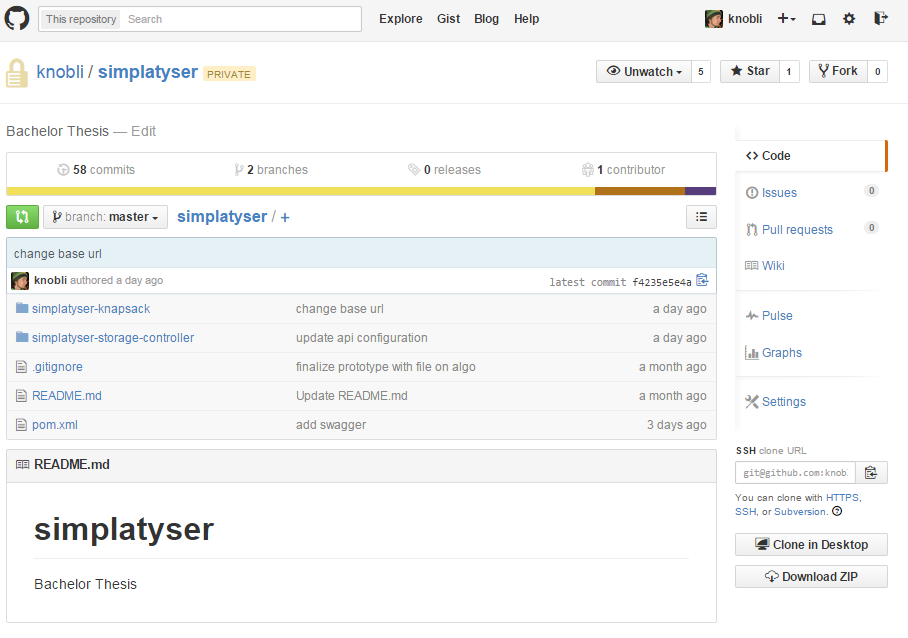
\includegraphics[scale=0.6]{images/github.png}
\caption[Github Repository des Simplatyser Projekts]{Github Repository des Simplatyser Projekts \selfmade{}}
\label{fig:github_repo}
\end{figure}

\FloatBarrier
\newpage

\subsection{Testen - Analysieren}
Über die Chrome App 'Advanced REST client' \cite{advanced_rest_client} (siehe Abbildung \ref{fig:advanced_rest_client})  wurde die Schnittstelle manuell getestet. Für die Regression-Tests 
wurde JUnit \cite{junit} und Mockito \cite{mockito} verwendet. Die statische Code Analyse wurde mit \gls{sonar} \cite{sonar} durchgeführt.

\begin{figure}[h]
\centering
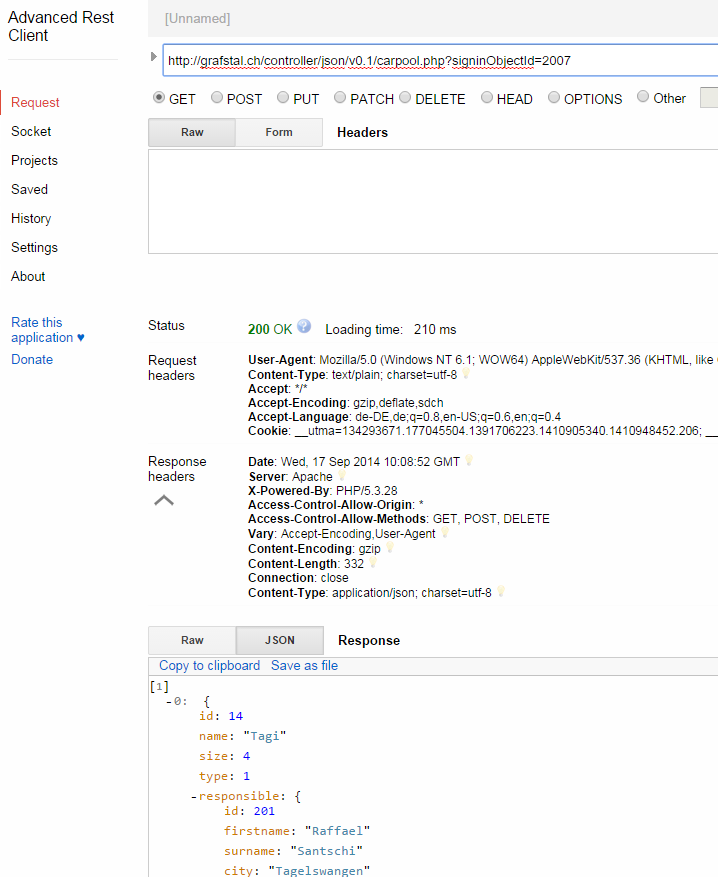
\includegraphics[scale=0.65]{images/advanced_rest_client.png}
\caption[Advanced REST client]{Advanced REST client \selfmade{}}
\label{fig:advanced_rest_client}
\end{figure}